\chapter{Playing for competitive advantage}\label{ch:playing_for_advantage}

As exposed in section~\ref{sec:dimensions}, one important dimension in the design of~\glspl{pirg} is that of playing for competitive advantage. This is not a special dimension of design present only in this type of application, but an intrinsic one necessary in all rational adversarial playing agents, both physical and virtual. Before designing the part of the system supporting  entertainment, which is the focus of our research and experiments, one must design the basic mechanism to enable the robot to take actions to win the game,~\ie take actions that satisfy the rules imposed by the game itself in the best possible way and act to profit of them -- which means being rational w.r.t the actions available in each game state. 

We recall that a low level of rationality shown by~\gls{pirg} agents is deemed to have negative impact on acceptability and fun~\citep{martinoia_physically_2013}. Playing for the purpose of human player entertainment in this scenario is not a trivial and can potentially have conflicting goals w.r.t. the objective of playing for competitive advantage. In general, one must trade-off the influence of the action planning in the general robot behavior so as to maintain a reasonable level of rationality while engaging players. In practice, this implies making a change in the utility function to incorporate aspects that make the game more enjoyable. Here, for our purposes, we decided to keep the two dimensions of play separate as depicted in figure~\ref{graph:PIRG_design_structure}. This allows for the modulation in playing for engagement while maintaining a working baseline for the competitive capability. Additionally, it makes up for easy code maintenance by separating the respective dimension requirements. In this chapter we describe how the robot plays for competitive advantage in our~\gls{pirg} scenario.

\section{Competitive advantage in RoboTower 2.0}\label{sec:competitive_adv_robotower2}

For our robot, action selection had at least three main concerns, namely: planning, timing and safety issues (see figure~\ref{graph:COMPETITIVE_structure}). The adopted planning algorithm was fast enough to provide the current best next tower to attack based on the current position of the robot and player with high frequency.

Although fast, for our game we had to constrain the system to take decision at a maximum frequency of 1Hz so as to help the player process better the game dynamics and have enough time to plan ahead and/or to rest. It became clear in the test phase that leaving the robot take decisions at a higher frequency would make the game very difficulty. Despite being a concern more related to the goal of playing for entertainment, the frequency constraint was considered necessary at this phase in order to make the game playable. 

\begin{figure}[H]
    \centering
    \begin{tikzpicture}[ every annotation/.style = {draw,
                         fill = white, font = \Large}, scale=0.75,transform shape]
                         
      \path[mindmap,concept color=black!40,text=white,
        every node/.style={concept,circular drop shadow},
        root/.style    = {concept color=black!40,
          font=\large\bfseries,text width=10em},
        level 1 concept/.append style={font=\Large\bfseries,
          sibling angle=60,text width=7.7em,
        level distance=15em,inner sep=0pt},
        level 2 concept/.append style={font=\bfseries,level distance=9em},
      ]
        node[concept, font=\fontsize{18pt}{17pt}\selectfont\bfseries] {Competitive\\Advantage}
        [clockwise from=0]
        % child[concept color=green!50!black] {
        %   node[concept] {Planning}
        %   [clockwise from=90]
        %   child { node[concept, scale=1, font=\fontsize{7pt}{17pt}\selectfont\bfseries] {World\\representation} }
        %   child { node[concept] {Hz} }
        %   child { node[concept] {Price} }
        %   child { node[concept, font=\fontsize{9pt}{17pt}\selectfont\bfseries] {Processing} }
        % }  
        child[concept color=blue] {
          node[concept] {Timing}
          [clockwise from=30]
          child { node[concept] {Reaction} }
          child { node[concept] {Actuation} }
        }
        child[concept color=red] {
            node[concept] {Planning}
            child { node[concept, scale=1.5, font=\fontsize{7pt}{17pt}\selectfont\bfseries] {World\\Modeling} }
            child { node[concept, scale=1.5, font=\fontsize{7pt}{17pt}\selectfont\bfseries] {Complexity}}
        }
        child[concept color=orange] { node[concept,font=\fontsize{14pt}{17pt}\selectfont\bfseries] {Safety}};
    \end{tikzpicture}
    \caption{Some relevant concepts in the competitive advantage dimension of a~\gls{pirg} agent.}
    \label{graph:COMPETITIVE_structure}
\end{figure}

Reaction time is an aspect that may be better explored by the system when playing for entertainment maximization, since it is an interesting feature to be evaluated in terms of potential contribution to the maximization of fun. For instance, the action planner may be modified to match the need to energetically react to in-game event, such as a surge of player activity aiming at attacking towers. In our research, the reaction time was explored in the study of deception and its contribution to the engagement in our~\gls{pirg} through the steering behavior approach for deception described in chapter~\ref{ch:deception}. In terms of competitive advantage, we maintained a constant reaction time to all in-game events.

Action selection occurred specifically by the implementation and testing of the~\gls{gob}~(\cite{millington_artificial_2009}) technique. This was possible due to the definition of attribute measures that help to decide the utility of actions; those were the human player \textit{current position} and all player's \textit{distance to towers}.

\glsdesc{gob} is a utility-based decision making procedure that can choose from a range of actions based on target goals. In our domain, our robot's set of goals, also called \textit{motives}~(\cite{millington_artificial_2009}), are defined as the necessity to be at a given location (the position of towers). To each goal, a level of importance is associated (often called \textit{insistence} in game design communities) and represented by a number. A goal with a high insistence will then tend to influence the robot's behavior more strongly. This approach makes the robot try to fulfill the goal in order to reduce its insistence. In our scenario, tearing down \textit{tower 1}, for example, is equivalent to reduce the insistence of the goal of going there (\verb|be_at_tower1|) to zero. 
%TODO Written like this it sounds strange. Maybe tearing down the tower will reduce the insistence of being there to 0. EWERTON: Done.

In addition, we need a suite of possible actions to choose from. These actions have the function of reducing insistence and direct the robot towards achieving goals. In our scenario, such actions are related to the actions of moving towards a known tower position. In terms of pseudo-code, our first approach for behavior selection was defined as follows~(\cite{millington_artificial_2009}).

\begin{lstlisting}[caption=A basic~\gls{gob} algorithm for action selection.]
def chooseAction(actions,goals):

  # Find the goal to achieve    
  topGoal = goals[0]
  for goal in goals[1..]:
    if goal.value > topGoal.value:
      topGoal = goal
    	
  # Find the best action to take
  bestAction = action[0]
  bestUtility = -actions[0].getGoalChange(topGoal)

  for action in actions[1..]:
    # We invert the change because a low changer value 
    # is good (we want to reduce the value for the goal),
    	# but utilities are typically scaled so high values 
    	# are good.
    		
    	utility = -action.getGoalChange(topGoal)
    		
    # We look for the lowest change (highest utility)
    	if thisUtility > bestUtility:
    	  bestUtility = thisUtility 
    	  bestAction = action
    			
  # Return the best action, to be carried out
  return bestAction
\end{lstlisting}\label{alg:planning}

The~\verb|getGoalchange()| method is responsible for accounting the reduction in insistence value for each goal. In our case, the utility function used for action selection in algorithm~\ref{alg:planning} is computed using attributes related to the player's interaction with in-game elements as well as to some robot attributes. We have defined a measure to account for the relationship between player's position and how much such position is contrasting the achievement of a goal by the robot.

We call this measure, player-tower \textit{blocking factor} $\Upsilon$, calculated for each tower  $\tau_{i},\forall i \in \mathcal{T}$, the set of towers, by equation~\ref{equation:utility_function}. 

\begin{equation}\label{equation:utility_function}
%\, produces a small space between elements
\Upsilon_{\tau_{i}} = \frac{atan2(\,
\sin(\,\left|\, \omega_{\tau_{i}}-\omega_{\rho}\right|\,),
\cos(\,\left|\,\omega_{\tau_{i}}-\omega_{\rho}\right|\,))}{\pi},
\end{equation}
 where $\omega_{\tau_{i}}$ denotes the angle between the robot's coordinate frame and the one of tower $\tau_{i}$, while $\omega_{\rho}$ denotes the angle between the robot's coordinate frame and the one of the player, respectively. The goal utility change produced by each action is then computed by the linear combination of the distance between the player and tower $\tau_{i}$ and $\Upsilon_{\tau_{i}}$. In order to create a more effective action selection procedure, we have decided to include also attributes like a scaled version of the number of charging~\glspl{led} in $\tau_{i}$ as well as robot's max speed for estimating time of arrival. Thus, for each tower $\tau_{i}$ we compose a vector whose components represent features of interest for the composition of the utility function as in~\ref{equation:utility_vector}.
 
\begin{equation}\label{equation:utility_vector}
\varphi_{i} = 
\begin{bmatrix}
    \delta(\rho,\tau_{i}) \\
    \Upsilon_{i}\\
    \lambda_{i}\alpha_{led}\\
    \delta(r,\tau_{i}),
\end{bmatrix}
\end{equation}
where $\delta(\rho,\tau_{i})$ represents the distance between human player $\rho$ and tower $\tau_{i}$; $\Upsilon_{i}$ represents the tower blocking factor; $\lambda_{i}$ the number of~\glspl{led}. A weight $\alpha_{led} \in \mathbb{R}$ is associated with $\lambda_{i}$ in order to regulate its importance. $\delta(r,\tau_{i})$, in turn, represents the distance between robot and tower.

One must recall that when defining an action selection procedure for~\gls{pirg} -- in the context of our research -- one is bounded by at least two different planning aspects: one associated with the game rules (which actions should the robot take next in order to win the game) and another with the maximization of fun (which action will maximize the player's fun, but at the same time not have a huge negative impact in the robot ability to be competitive) The utility description presented here only considers the first aspect. From chapter~\ref{ch:activity} onward we aim at providing some direction to the second aspect in a way that it is general enough to be applied in many different situations. 

Safety was also a limiting factor in the context of playing for competitive advantage; as said previously, the maximum velocity of our mobile platform had to be limited not only from the perspective of game mechanics, but by the imminent probability that a player would eventually collide against it when fighting for a tower. Precisely, the velocity of which to go towards a tower had to be capped by a maximum value so as to be managed appropriately by the velocity smoothing algorithm and obstacle avoidance sub-system%TODO What does this mean? %EWERTON: Not all velocities can be used with out obstacle avoidance: Put too much velocity and you risk colliding the robot or mechanically breaking it down.
. While this gives enough control of the platform so as to make it play %giving the platform enough condition %TODO What does this mean? % EWERTON: I Modified the text. Please, see whether you like it.
without physically endangering the human player, limiting the velocity of the robot can give away its intentions and harm the ability to be competitive. For the purpose of behavior adaptation when playing for human entertainment maximization, we have determined discrete values for the variable describing \textit{velocity}, \textit{acceleration} and \textit{blocking factor} such that different safe playing styles could be adopted. This discrimination is going to be object of chapter~\ref{ch:adaptation}.

In general, our research concentrated in providing insights for the adaptation of robot behavior for the purpose of entertainment support through latent~\gls{ml}-based models and difficulty selection. Therefore, we worked mostly in the dimension discussed in section~\ref{sec:dimensions}, thus, keeping fixed the ability to play for competitive advantage to what described above. In the next section we bring up a brief review of literature regarding systems that perform player modeling for competitive advantage in video-games. Despite not being a thorough review on the subject, the section provides a good overview, being useful for designers who want to target this dimension.

%TODO It is quite strange to have a review after the presentation of what is done. I recognize it is interesting, but a review should be related to what has been done. A relationship between something of what presented below (that should go before) and your choices should be done. STILL TO BE FIXED
% EWERTON: I think this is useful anyway. We haven't done anything in terms of playing for competition (it was not the object of our research). However, I wanted to give the reader a broad overview of approaches to this matter. I did not placed it at the beginning because of this very same reason. It is here as a plus, an optional reading for the ones interested to know more about this subject. What do you suggest doing with it now? 

\section{Player modeling for competitive advantage in video-games}\label{compadvantage}
There is a set of different lines of research that examine several different methods and goals by which an autonomous system, either virtual or robotic, can learn to recognize activities. Here, we focus on systems that exhibit some concerns about taking advantage from knowledge extracted from physical interaction in robotic competitive environment and virtual scenarios. Since the adversarial nature, these methods are often referred to as approaches that use \textit{opponent modeling}. Specifically, this section summarizes prominent aspects of popular opponent modeling papers envisioning to point out related possibilities for~\gls{pirg} design. I begin by stating the basic work-flow that is often done when constructing such approaches. 

Commonly, three basic steps are followed: \textit{feature extraction, model construction, and design of changes} as shown in Figure~\ref{behaviorModWorkFlow}. Feature extraction relates to the idea of choosing which set of raw sensory inputs (or their combination) gives most information for capturing features of the user behavior. Once the features have been identified, a model is constructed to support any successive user classification attempt. Intuitively, the goal here is to design a way to get models of the different types of behavior/strategy co-playing agents (opponent) might have, thus enabling recognition. The last step is the decision about how the system should react to different users. This is undoubtedly the most difficult phase since, among other things, adjustments should also take into consideration the effect of modeling errors. Perhaps, the reader could realize that this work pipeline is similar to approaches normally used in data mining or statistical/machine learning methodologies.

\begin{figure}[htp]
  \centering  
  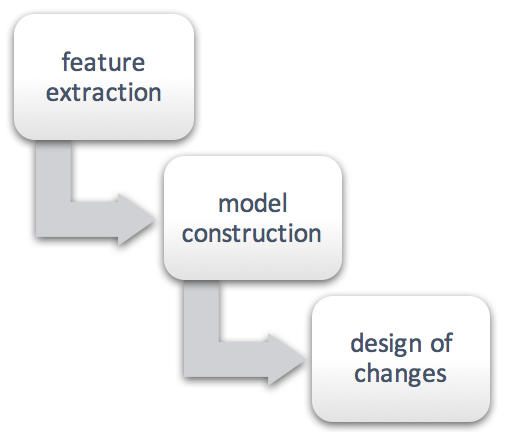
\includegraphics[draft=false,scale=0.6]{images/02-art/oppmodelproc.png}
  \caption{Basic work-flow for designing systems able to implement any kind of modeling of co-existing agents for competitive advantage.}
   \label{behaviorModWorkFlow}
\end{figure}

It is not a secret that in order to be able to increase the likelihood of winning a game one should also consider the extraction of knowledge from opponents in the environment. Opponent modeling \textit{per se} is seen as the attempt to predict and identify behaviors of co-existing adversarial agents and propose appropriate countermeasure actions toward maximizing a given utility~\citep{fathzadeh_opponent_2007}.

In the Robot World Cup Initiative (RoboCup) a body of research has been done in the last decade trying to address the problem of opponent modeling. The RoboCup is a multidisciplinary initiative for building, among other, a team of robots capable of playing soccer. In this scenario, opponent modeling concepts are seen as an important requirement for building a competitive team and also as a growing research topic not only on this domain but also in the more general multi-agent system area~\citep{rofer_overview_2012}. 

Since in most cases game history data is available, researchers have extensively used data mining and~\gls{ml} techniques in order to construct off-line models of opponents which could then be used as classes in a kind of ``prediction phase'' during actual game play. Often, this prediction phase basically means: try to match the current observed opponent behavior to one the existing models for then try to adjust the internal behavior parameters accordingly. This matches the basic work-flow scheme in figure~\ref{behaviorModWorkFlow}.

Some important contribution to the problem has been proposed by~\citep{fix_behavior_2000,riley_recognizing_2002,riley_coaching_2001,riley_planning_2002}. In~\cite{riley_recognizing_2002}, the authors explored the domain of RoboCup by studying how to improve their agent team by constructing a probabilistic model representing predicted opponents' locations given the recent history of ball's movement and initial team members' locations. As common in this scenario, their approach focused in the use of a ``coach'' agent, enabled with a number of predefined models and a centralized view of the world, whose main role is that of communicating a plan to the rest of the team. The big idea is to take into consideration how a model matches the observed data in order to predict the opponent general behavior. 

The main assumption made by the author was that the opponent behavior can be generated from a sample drawn from the predefined set of models given to the coach. Given the predefined models, it is a challenge to decide which model best describes the opponent at run-time. As in the common supervised learning paradigm, they assumed the opponents will behave similarly to how they performed in the past, and use that information to develop a plan. In all of the models used, the distribution of each player's final position was represented by a two-dimensional Gaussian with equal variance in all directions. On successive works~\citep{riley_coaching_2001,riley_planning_2002} the authors managed to improve the online model selection through a kind of Naive Bayes approach focusing on plan representation and execution expressing spatial-temporal relations. 

An interesting observation made by the authors, also pointed out in the work of ~\cite{rofer_overview_2012}, is that during the plan execution it was not possible to take advantage from single unpredictable opportunities that may emerge. For instance, the agents would follow the plan strictly even if there is a clear chance of being successful against the opponent team by taking an immediate off-plan action. It is important to observe how this issue may direct affect the efficiency of an autonomous agent involved in a~\gls{pirg}. It is extremely necessary for the agent to keep a closer loop with the environment, paying attention to every observation that may emerge, as opposed to follow blindly a pre-selected behavior. Naturally, this paves the road for solutions that can represent some degree of belief regarding plan execution and revision. A possible solution to this issue was also pointed out by the authors. They basically suggested to store alternative plans and intelligently add monitors for these plans as in~\cite{veloso_rationale-based_1998} so that they could make the plan execution opportunistic~\citep{riley_coaching_2001,riley_planning_2002,rofer_overview_2012}.

In~\cite{iglesias_comparing_2006} the goal was to use statistical dependency tests for the identification of significant sequences from which to relate states to chains of events. Their underlying assumption was that observed team behavior can be transformed into a sequence of ordered atomic behaviors. In the follow-up work~\cite{burgard_classifying_2008}, sub-sequences inside sequences of behaviors are analyzed by using a frequency-based method. The most relevant aspect presented on their work is that the model of an agent behavior is represented by a distribution of relevant sub-sequences. The behavior classification procedure is done using a modified Chi-square Test.

\cite{steffens_feature-based_2003} studied the application of feature-based models for representing opponent behavior. The gist of this approach is the identification of few features that could be observed by raw sensor data during game play, which diverged from~\cite{fix_behavior_2000} who stored every observation on the model. These features were classified by using a Bayesian method, then a knowledge base is used in order to respond to what has been classified, i.e, select the appropriate strategy. One example of such features were text-based description for in-game situations, like: ``The opponent often does long passes along the left wing to the forwards''. The methodology investigated in the paper was further studied in the context of Case-based Reasoning in~\cite{steffens_similarity-based_2005}. In this follow-up research, Steffens was able to identify some gain in classification accuracy showing that similarity-based opponent modeling could benefit from domain knowledge~\citep{rofer_overview_2012}. Case-base Reasoning, however, is likely to lead to high computational costs given the large number of cases to be retained in a highly dynamic environment~\citep{ahmadi_using_2004,rofer_overview_2012}.

\cite{kaminka_learning_2003} translate observations into a time-series of recognized atomic behaviors. For instance, given a stream of raw observations about the team members' position and orientation plus the position of the ball, their approach would recognize soccer-playing behaviors (passes, dribbles, etc.). Unlike other efforts, they did not care about how the low-level behaviors combine together for generating high-level strategies.  

\cite{ledezma_predicting_2002} also formulates the problem of opponent modeling as a classification task. In tackling the problem they proposed the decomposition of the learning task into procedures: the learning of the action name (passing the ball, kicking), and learning the parameters of the action. A follow-up work~\citep{ledezma_predicting_2005} further studied the subject by implementing~\gls{ml}-based methods to create modules that are able to infer the opponent's actions by means of observation. Their method, was called ``Opponent Modeling Based on Observation'' (OMBO) and was designed to make improvements along two pathways: First, tackling the creation of a generic module (Action Labeling Module) that is able to label the last action (and its parameters) performed by any robosoccer opponent. This happens via the observation of another agent. The justification for this method is that agents generally do not have access to input/output pairs of events generated by other agents. So, the approach must rely on sensor inputs only. Second, the construction of a model of the other agent is based on data acquired from the first module. This is what they called ``Model Builder Module''. In ~\cite{ledezma_ombo:_2009} they further discussed the applicability of the OMBO method giving a proof-of-concept of learning a model of two different goalies. The idea was that their team striker gets as close to the goal as possible, and shoots when the goalie is predicted to move, i.e, by anticipation of the opponent movement. Figure~\ref{OMBO_model_task} presents the holistic view of the method found in~\cite{ledezma_predicting_2005,ledezma_ombo:_2009}. 

\begin{figure}[htp]
  \centering  
  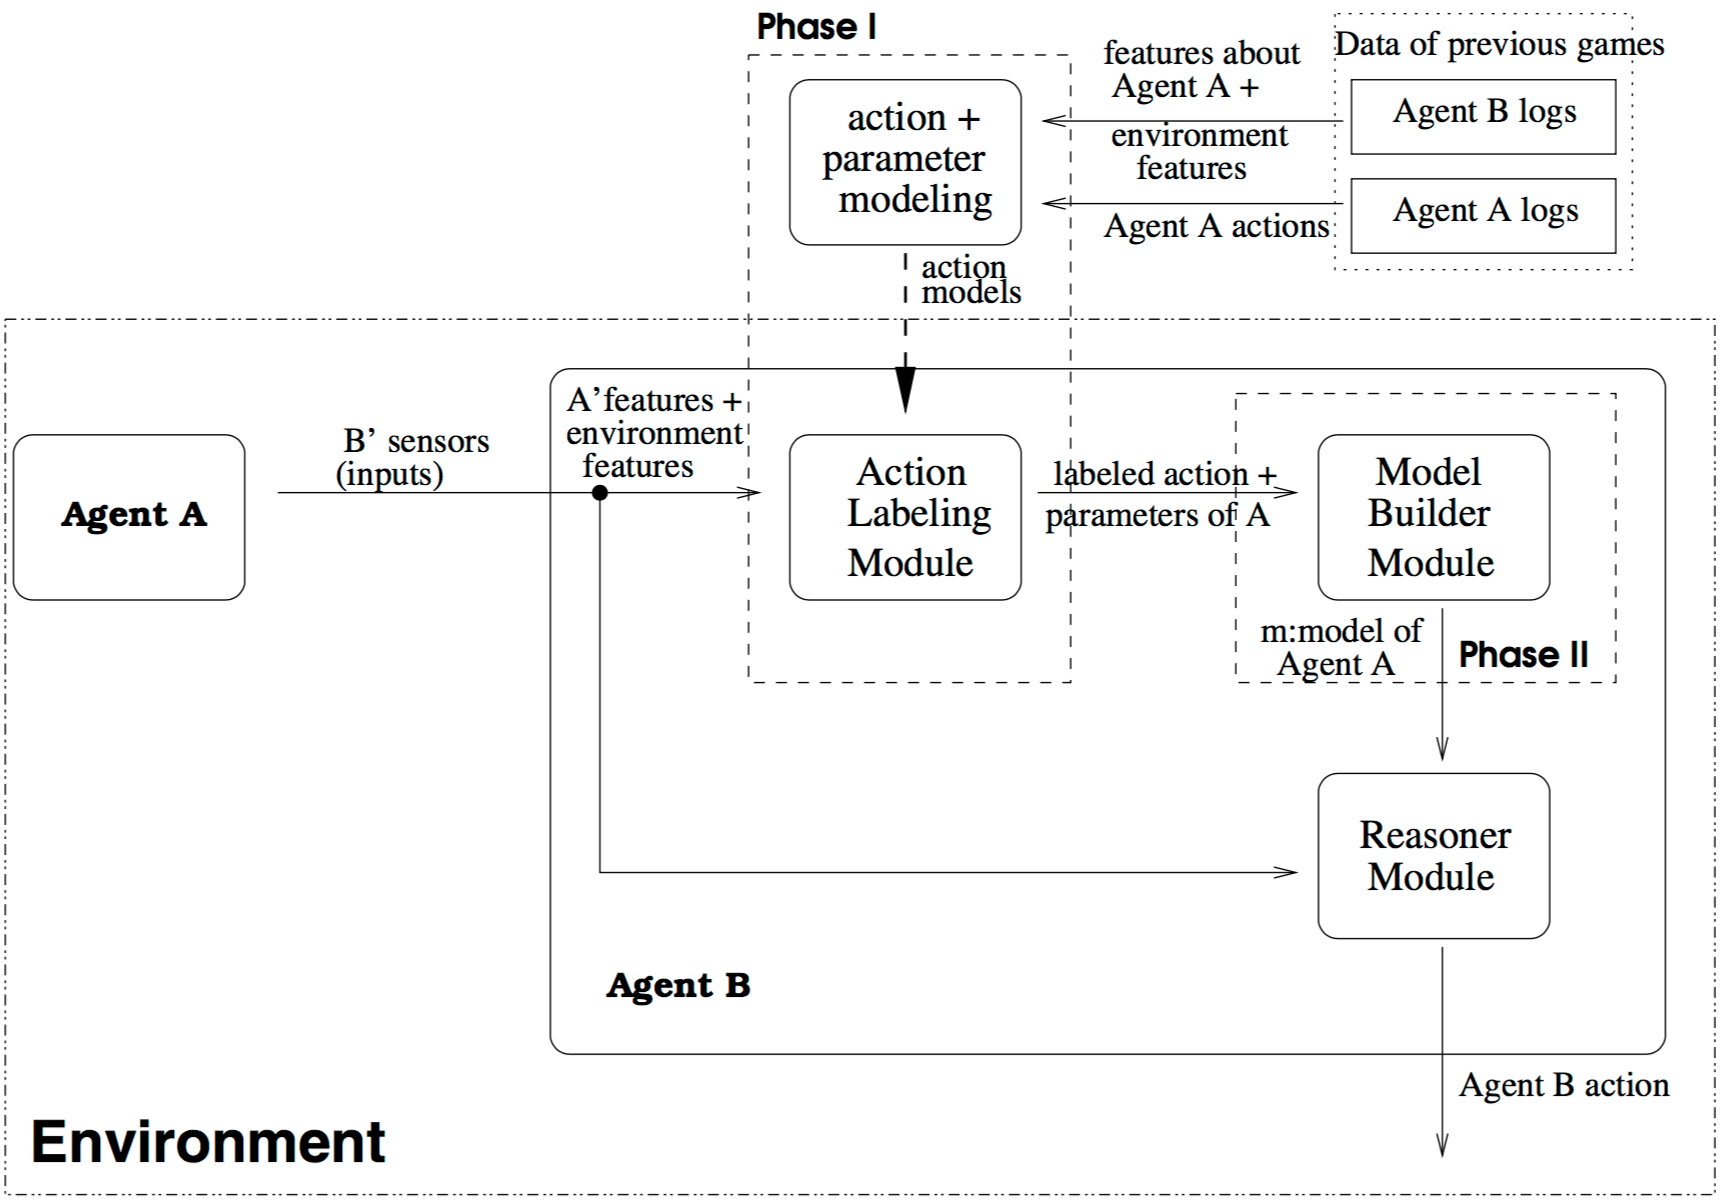
\includegraphics[draft=false, width=\textwidth]{images/04-competition/OMBO_model_task.png}
  \caption{The OMBO model from~\cite{ledezma_predicting_2005, ledezma_ombo:_2009}. The approach is based on two main phases: action labeling and model building.}
    \label{OMBO_model_task}
\end{figure}

Using data mining in order to define models of opponents in an off-line manner is the ideal scenario of an agent learning a model of other agents' behavior via direct observation of their past actions. However, this is only reliable when agents have many repeated interactions with one another or when the assumption of similar behavior between agents holds, otherwise it is hard to obtain any good generalization~\citep{stone_defining_2000}. Given the characteristics of the domain (physical interaction between agents), one may realize that the notion of proximity is quite important\footnote{Proximity is a notion that basically relates to how close/distant are interacting entities. It this turns out to be an ubiquitous notion even in simulated physical interaction as that showed in most videogames.}. Often, authors try to exploit proximity aspects as well as the spatial-temporal relations with certain property of the environment, for instance, the domain an agent exert over a field region (e.g,~\cite{riley_empirical_2002}). Obviously, proximity is not enough, but when combined with other aspects, like timing aspects, it is possible to get good estimates about the behavior of agents in their attitude with respect to in-game tasks. This trend is going to be present on the majority of papers focusing behavioral modeling.

Using the Rush 2008 American football simulator,~\cite{laviersa_using_2014} introduced methods for performing predictions about the players' physical movements when learning team policies. When focusing on recognition of team play they investigated the use of~\gls{svm}, an optimal margin classifier commonly used in supervised learning problems. They trained~\glspl{svm} for a multi-class objective by using a collection of simulated games under controlled conditions, so they got instances of every possible combination of offense and defense plays from a number of team starting formation configurations. The output of the play recognizer was defined as the system's best guess (at the current time step) about the opponent's choice of defensive play. Thus, they could use this information to select the most appropriate offense.

Also in~\cite{laviersa_using_2014}, the authors focused on proposing methods for discovering how to effectively  subgroup agents together so to accomplish a given formation task, similar to~\cite{stone_task_1999}. Here again they based their method on an analysis of game data from successful team plays. The idea was to implement a supervised learning mechanism in order to identify important groups of players in each play. It is interesting to mention the three general types of cues that were used for the purpose of subgroup extraction: \textit{spatial} -- i.e, the constant relationships between team members over a period of time; \textit{temporal} -- co-occurrence of related actions; \textit{coordination} -- dependencies between members' actions. These cues turn out to be basics features for most types of approaches in the discussed scenario.

When tackling team formation, one may observe that a large number of~\gls{ml} techniques have been tested in order to improve countermeasures for a specific team. Again, most of the methodologies use log files for the purpose of off-line learning of relevant characteristics. Neural Networks, for instance, have been extensively used for identifying the position of opponent team members with respect to given preset formations. After identifying a given formation, a plan could be transmitted by the coach agent to the rest of the team all for the purpose of performing the appropriated counteraction~\citep{nakashima_off-line_2010,ramos_discovering_2008, faria_machine_2010, visser_recognizing_2001}.

For a in-depth overview of opponent modeling in RoboCup the reader is invited to refer to~\cite{rofer_overview_2012}. In the work the authors classify methodologies into two categories which basically comprise \begin{inparaenum}[\itshape a\upshape)]\item``formation modeling'', as it stands for the task of modeling team plays under the umbrella of collective behavior, and \item``individual behavior modeling'', which is related to the idea of modeling a single opponent agent\end{inparaenum}.

%TODO You cannot limit this important section to the summary of an old paper reporting older results. I cannot believe there aren't any other approaches to model opponents for competitive advantage.
% EWERTON: I can try to insert more as soon as I solve the other more urgent issues in the text. 

\subsection{Commercial interactive simulated environments}

Virtual games have enabled a large amount of research effort into the design of player modeling methodologies. This is due to the increasing need for making~\gls{npc} believable, i.e, make them resemble human behavior by implementing similar (to human) deductive reasoning process for action selection. In summary, the need of such ability in virtual games is at least due to a few main facts: \begin{inparaenum}[\itshape a\upshape)]\item the growth as a commercial product; \item the increasing complexity; as well as \item the need for developing games that can exhibit a major level of intelligence and adaptation (personalization)\end{inparaenum}~\citep{bakkes_personalised_2012}. 

A growing collection of papers have been published trying to address the problem of predicting the player (opponent) behavior (actions) in different levels and in different contexts. Focusing on opponent modeling, \cite{herik_opponent_2005} presented an overview of efforts for commercial games. In this work, they emphasize types and roles of opponent models, such as ``speculation'', ``tutoring and training'' as well as ``mimicking characters''. In ``speculation'', the idea is that some kind of heuristic (or utility function) -- such as minimax in zero-sum games like chess or checkers -- is used in order to assess the quality of available opponent's actions during game-play. In simple terms, this relates to the idea of using knowledge of the opponent's preferences or skills in order to drive the game into positions/states that are considered to be \textit{less favorable} to the opponent. This is the same core idea behind the approach described in~\cite{markovitch_learning_2005}, where they defined the concept of \textit{opponent weakness} (as a quantifying measure) together with a method for learning a model of this concept. The key-point in~\cite{markovitch_learning_2005} was the care about the potential harm of modeling error and the incorporation of their concept as an extra feature in the decision process, not as the core itself.

Another example of such modeling type is the research done by~\cite{missura_online_2008}, where the authors propose to rank available actions for the player (at each turn of the connect four game) to find a way to balance the behavior of the computer-controlled agent to that of the human player. The aim was to estimate the player's expertise, when looking at the history of moves performed, and by assessing their quality (rank) based on a minimax approach.  Thus, at each turn, they could make their agent select only actions that have similar rank to that of the player\footnote{Despite the fact~\cite{missura_online_2008} is mentioned here as a ``speculation'' type of opponent modeling -- since there is a kind of simulation procedure for evaluating the player's quality of movement -- one may also see this work as an effort for tailoring the game for optimizing gaming experience, i.e., a kind of difficult adjustment approach.}.

Tutoring and Training is seen in~\cite{herik_opponent_2005} as a type of opponent modeling that has to do with the assistance of a human player. For instance, a model of the human opponent may be built as to teach him how to achieve certain in-game goals in a personalized manner. This is ideal for \textit{serious game} environments where the player is confronted with a simulation of real-world events while trying to solve a potential real-world problem. Even by knowing that serious games can be entertaining, in this scenario the main purpose is essentially to train or educate users, thus, coming up with models that support the game steering behavior towards those aspects that are definitely important. In this context, \cite{ha_goal_2011} tried to identify player's goals in the Crystal Island game -- a non-linear educational game about microbiology -- by using Markov Logic Networks\footnote{A probabilistic technique comprising a set of weighted first-order logic \textit{formulae} that enables uncertain inference over Boolean logic. }. Goal recognition is assumed to be an important piece for player modeling and generally tries to identify the user's goals from a set of low-level observation (abduction)\footnote{Also related to goal recognition are techniques like plan and activity recognition, both well-known problems in general~\gls{ai}~\citep{ha_goal_2011}.}. 

The study in~\cite{ha_goal_2011} follows previous work on goal recognition (such as~\cite{mott_probabilistic_2006}), but under a much broader view, that of having individual goals not independent from each another (which turns goal recognition into a classification problem) and that of having ambiguous causality effect between actions and goals. In terms of features for player actions, they targeted three properties: \textit{action type} (e.g, moving to a place), \textit{location} (game place where the action was taken), \textit{narrative state} (player's progress in the game narrative).  Once again, model parameters are learned from corpus of data collected from the environment. Their results were compared with two baselines based on \textit{unigram} (a model that predicts goals based on the current player action) and \textit{bigram} models (makes prediction based on previous action as well) obtaining a 82\% improvement over them.

In~\cite{herik_opponent_2005}, the ``mimicking characters'' type is said to correspond to the observation that the virtual game is designed to be fun and entertaining, as opposed to play as strong as possible all the time. This amounts to the well-known observation that when performing a companion role, for example, the agent must do what is possible to behave in accordance to the expectation of the player, otherwise the human may lose interest in the game. Thus, this requires a model of the human in order to be effective. Also, in a~\gls{pirg} scenario, this is an important aspect that would enable advancements in the interaction as a whole since the behavior of an autonomous agent should be dynamic enough to adjust to the individual experience. The central point is that of not designing static behaviors that are likely to be exhaustively exploited by the player. This type hugely overlap with the ideas of player modeling for creating a balanced game play, i.e., adjusting the game for the player individual experience. This subject is brought back on section.  

Often, games and simulations provide access to full-observability of in-game events and player's actions. When this is not true, there may be a (often large) corpus of data from usage history that is available for information extraction. This, naturally favors the use of off-the-shelf data-mining algorithms that can be easily set up and tested multiple times. However, on the design of~\gls{pirg}, specially on a brand-new project, one may suffer from the lack of data for constructing off-line models of players. To get around this problem there exist at least two main alternatives: \begin{inparaenum}[\itshape a\upshape)]\item setup a data collection procedure, for example, by designing a first version of the game, implementing it and then collecting data in order to refine the game design; or \item invest on online procedures that are able to extract features from the player and come up with models of player behavior on run-time\end{inparaenum}.

In~\gls{pirg}, it should be possible to design methods that account for the evaluation of the current state in order to know what are the corresponding chances of winning/losing at the moment, allowing for planning ahead how to overcome/support in case of need. However, it is worth to take into account the general constraints perceived in the domain, such as computing complexity, mobility and perception constraints. 

Moreover, there is to consider that computation in~\gls{pirg} should be supported by low cost platforms only, which have limitations in computing power, energy consumption and other.

\section{Considerations}
In this chapter we have described the concepts behind our platform's ability to play competitively,~\ie to select actions aimed at winning the game. We have kept this goal separate from that of modeling player for the purpose of entertainment maximization, and of driving the robot behavior towards this, since we view the two goals as often conflicting. While ideally we search for a robot that is able to act rationally under the later objective, it should also provide means for competitively engaging the player and obey the game rules. In theory, the robot should tend to balance its chances of winning the game with the player's ones. However, it should not do that in a way that can be interpreted by the player as ``letting'' him win. Therefore, in our experiments we decoupled the two styles of playing in order to easy tackle each style issues and concerns individually. For all factors, our work assumed the robot's ability to play the game well enough to be perceived as a competitive agent and we did not deal much with this dimension. This assumption was confirmed in the self-report given by players after the game. In the next chapters we present the contributions of our research in modeling the player for entertainment maximization.